
\newpage
\section{Definitions and Overview}\label{sec:2}

XAI, short for Explainable Artificial Intelligence, is a term often used in the field of machine learning. It's all about going beyond a mysterious "black box" approach and aiming to understand how a trained model makes decisions.\\
In this chapter, we'll explore the uses of ML Interpretability. Next, we'll examine the different forms in which explanations can be presented. Finally, we'll categorize the types of machine learning models and algorithms.

\subsection{Goals of ML Interpretability}\label{sec:goals}

\subsubsection*{Justify the model} 
The main aim of XAI is to make models easy to understand so that people can trust them more and feel confident in their predictions. This means making the model transparent so that we can understand how it makes its predictions.

According to \cite{InterpretableToWhom}, it's also important to consider who needs the explanation. Different people play different roles in how machine learning systems work.
In a machine learning ecosystem they define six roles, illustrated in Figure \ref{fig:InterpretableToWhom}, where individuals may fulfill more than one role simultaneously.

\begin{figure}[H]
    \centering
    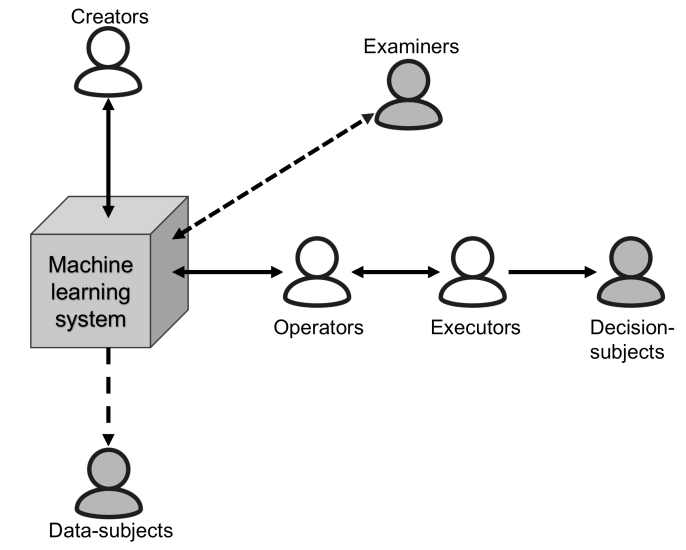
\includegraphics[width=0.6\linewidth]{pics/ill_ml_justify.png}
    \caption{Illustration of a machine learning ecosystem.\cite{InterpretableToWhom}}
    \label{fig:InterpretableToWhom}
\end{figure}

First, there are the creators who build and develop the machine learning model. Then, there are the operators who manage and run the model once it's implemented. Next, there are the executors who use the model to make decisions. After them, there are those who are impacted by the decisions made by the executors. This includes people whose personal data was used to train the model, as well as those who audit or investigate the machine learning system.

Understanding these different roles helps ensure that explanations are useful and relevant to everyone involved.

\subsubsection*{Get insights into data}
Another aim in XAI is to gain insights from the data. Instead of just focusing on the model, the goal is to understand how the real-world process operates and how the features relate to the target. 
However, achieving this goal heavily relies on the model's performance. For XAI to be effective in uncovering insights, the model must perform well.\cite{freiesleben2022scientific}

\subsubsection*{Debug and improve model}
One of the aims of XAI is to find and fix mistakes or unfairness in models and data. This involves spotting things like missing values or repeated information in the dataset, shifts in the data over time or finding redundant features that don't add any new useful information.\cite{hassija2024interpreting,InterpretableToWhom}

\subsection{Different forms of explanations}

XAI approaches can provide various types of explanations.

\subsubsection*{Features statistics + visualization}
One form of explanation involves offering feature statistics, which can often be represented visually. For example, techniques such as Permutation Feature Importance (T. \ref{tab:XAIPFI}) or Shapley values (T.\ref{tab:XAIShapVal}) provide importance metrics indicating the influence of each feature on the model's prediction. Certain feature explanations are best understood through visualization, such as the saliency map produced by the Vanilla Gradient method (T.\ref{tab:VanillaGradient}).

\subsubsection*{Internal parameters of a model}
Another form of explanation involves gaining insight through internal model parameters. For instance, this can be observed in the weights of Linear Regression models (T. \ref{tab:XAILinReg}), which serve as both feature statistics and components of the model's internal workings. Similarly, the internal structure of Decision Trees (T. \ref{tab:Tree}) offers valuable insights into how the model makes decisions.

\subsubsection*{Points from dataset distribution}
This form of explanation includes all approaches that uses data points from the existing data distribution or newly generated data points to improve model interpretability. For example, the model utilizes available data points from the dataset to make predictions, like with the ProtoPNet architecture discussed in subsection \ref{sec:ProtoPNet}.

\subsubsection*{Approximation of model with an inherently interpretable model}
Another form of explanation involves approximating a complex model with an interpretable one, either a globally using a global surrogate (T. \ref{tab:XAIGlobSur}), or locally as seen in methods like LIME (T. \ref{tab:XAILIME}). This interpretable model can then be analyzed by examining its internal parameters or interpreted by obtaining feature statistics.
% Another form of explanation is to approximate a complex model with an interpretable model, either globally with a global surrogate or locally for e.g. LIME. The interpretable model itself is interpreted by either looking at internal model parameters or feature statistics.

\subsection{Taxonomy of Explainable AI Approaches}

The taxonomy of XAI approaches is illustrated in the following figure:
\begin{figure}[H]
    \centering
    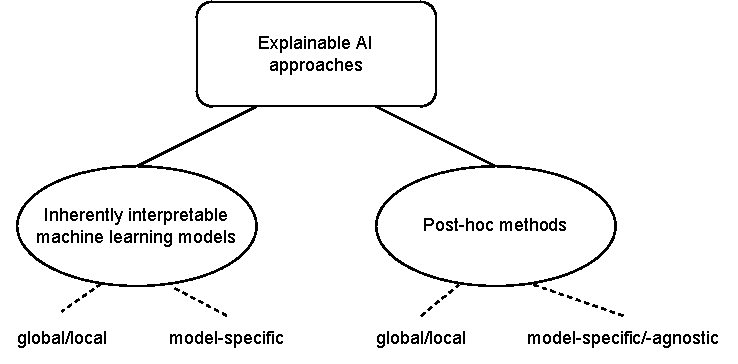
\includegraphics[width=0.85\textwidth]{pics/XAI_Overview.pdf}
    \caption{Overview over XAI.}
    \label{fig:ov-xai}
\end{figure}

XAI approaches can be divided into two main types. Firstly, there are \textbf{inherently interpretable ML models}, characterized by either a straightforward structure that is easy to interpret or models where interpretability is integrated into the architecture itself. Secondly, there are \textbf{Post hoc Methods}, which are applied to trained models. \\
An important distinction to note is whether the approach entails global or local interpretability. \textbf{Global interpretability} aims to comprehend the overall behavior of the model in making predictions. For instance, in a Linear Regression model, insights can be derived by analyzing the weights, while in a Decision Tree, one can analyze the nodes to understand the prediction mechanism. On the other hand, \textbf{local interpretability} aims to understand the reasoning behind individual or grouped predictions. \\
Furthermore, another important distinction is whether an approach is model-specific or model-agnostic. \textbf{Model-specific} approaches work only with particular model classes. Inherently interpretable ML models fall into this category by design. Additionally, post-hoc methods can also be model-specific, such as the Vanilla Gradient method (T. \ref{tab:VanillaGradient}), which is only applicable to models allowing gradient computation.
Conversely, \textbf{model-agnostic} approaches are post-hoc methods capable of being applied to any model.
